\newcommand{\svcourse}{CST Part IA: Software Engineering and Security}
\newcommand{\svnumber}{1}
\newcommand{\svvenue}{Microsoft Teams}
\newcommand{\svdate}{2022-05-11}
\newcommand{\svtime}{15:00}
\newcommand{\svuploadkey}{CBd13xmL7PC1zqhNIoLdTiYUBnxZhzRAtJxv/ytRdM1r7qIfwMsxeVwM/pPcIo8l}

\newcommand{\svrname}{Dr Sam Ainsworth}
\newcommand{\jkfside}{oneside}
\newcommand{\jkfhanded}{yes}

\newcommand{\studentname}{Harry Langford}
\newcommand{\studentemail}{hjel2@cam.ac.uk}


\documentclass[10pt,\jkfside,a4paper]{article}
\usepackage{amsfonts}
\usepackage{mathtools}
\usepackage{graphicx}
\usepackage{textcomp}
\usepackage{float}

% DO NOT add \usepackage commands here.  Place any custom commands
% into your SV work files.  Anything in the template directory is
% likely to be overwritten!

\usepackage{fancyhdr}

\usepackage{lastpage}       % ``n of m'' page numbering
\usepackage{lscape}         % Makes landscape easier

\usepackage{verbatim}       % Verbatim blocks
\usepackage{listings}       % Source code listings
\usepackage{graphicx}
\usepackage{float}
\usepackage{epsfig}         % Embed encapsulated postscript
\usepackage{array}          % Array environment
\usepackage{qrcode}         % QR codes
\usepackage{enumitem}       % Required by Tom Johnson's exam question header

\usepackage{hhline}         % Horizontal lines in tables
\usepackage{siunitx}        % Correct spacing of units
\usepackage{amsmath}        % American Mathematical Society
\usepackage{amssymb}        % Maths symbols
\usepackage{amsthm}         % Theorems

\usepackage{ifthen}         % Conditional processing in tex

\usepackage[top=3cm,
            bottom=3cm,
            inner=2cm,
            outer=5cm]{geometry}

% PDF metadata + URL formatting
\usepackage[
            pdfauthor={\studentname},
            pdftitle={\svcourse, SV \svnumber},
            pdfsubject={},
            pdfkeywords={9d2547b00aba40b58fa0378774f72ee6},
            pdfproducer={},
            pdfcreator={},
            hidelinks]{hyperref}

\renewcommand{\headrulewidth}{0.4pt}
\renewcommand{\footrulewidth}{0.4pt}
\fancyheadoffset[LO,LE,RO,RE]{0pt}
\fancyfootoffset[LO,LE,RO,RE]{0pt}
\pagestyle{fancy}
\fancyhead{}
\fancyhead[LO,RE]{{\bfseries \studentname}\\\studentemail}
\fancyhead[RO,LE]{{\bfseries \svcourse, SV~\svnumber}\\\svdate\ \svtime, \svvenue}
\fancyfoot{}
\fancyfoot[LO,RE]{For: \svrname}
\fancyfoot[RO,LE]{\today\hspace{1cm}\thepage\ / \pageref{LastPage}}
\fancyfoot[C]{\qrcode[height=0.8cm]{\svuploadkey}}
\setlength{\headheight}{22.55pt}


\ifthenelse{\equal{\jkfside}{oneside}}{

 \ifthenelse{\equal{\jkfhanded}{left}}{
  % 1. Left-handed marker, one-sided printing or e-marking, use oneside and...
  \evensidemargin=\oddsidemargin
  \oddsidemargin=73pt
  \setlength{\marginparwidth}{111pt}
  \setlength{\marginparsep}{-\marginparsep}
  \addtolength{\marginparsep}{-\textwidth}
  \addtolength{\marginparsep}{-\marginparwidth}
 }{
  % 2. Right-handed marker, one-sided printing or e-marking, use oneside.
  \setlength{\marginparwidth}{111pt}
 }

}{
 % 3. Alternating margins, two-sided printing, use twoside.
}


\setlength{\parindent}{0em}
\addtolength{\parskip}{1ex}

% Exam question headings, labels and sensible layout (courtesy of Tom Johnson)
\setlist{parsep=\parskip, listparindent=\parindent}
\newcommand{\examhead}[3]{\section{#1 Paper #2 Question #3}}
\newenvironment{examquestion}[3]{
\examhead{#1}{#2}{#3}\setlist[enumerate, 1]{label=(\alph*)}\setlist[enumerate, 2]{label=(\roman*)}
\marginpar{\href{https://www.cl.cam.ac.uk/teaching/exams/pastpapers/y#1p#2q#3.pdf}{\qrcode{https://www.cl.cam.ac.uk/teaching/exams/pastpapers/y#1p#2q#3.pdf}}}
\marginpar{\footnotesize \href{https://www.cl.cam.ac.uk/teaching/exams/pastpapers/y#1p#2q#3.pdf}{https://www.cl.cam.ac.uk/\\teaching/exams/pastpapers/\\y#1p#2q#3.pdf}}
}{}


\begin{document}

\begin{enumerate}

\item

Suppose that $X$ is a random variable with the $U(-1, 1)$ distribution.
Find the exact value of $\mathbb{P}(|X| \geq a)$ for each $a > 0$ and
compare it to the upper bounds obtained from the Markov and Chebyshev inequalities.

If $X$ is a random variable with the $U(-1, 1)$ distribution, then $|X|$ is a random variable with the $U(0, 1)$
distribution. We can therefore use the probability density function, expectation and variance of a uniform
distribution in subsequent parts of the question.

\[
\mathbb{P}(|X| \geq a) =
\begin{cases}
1 - a & \text{ if } a \geq 0 \\
0 & \text{ otherwise }
\end{cases}
\]

Using Markov's inequality:
\[
\begin{split}
\mathbb{P}(|X| \geq a) &\leq \frac{\mathbb{E}(|X)}{a} \\
&\leq \frac{\frac{1}{2}}{a} \\
&\leq \frac{1}{2a} \\
\end{split}
\]

Using Chebyshev's inequality:
\[
\begin{split}
\mathbb{P}(||X| - E[X]| \geq x) &\leq \frac{Var(X)}{x^2} \\
\mathbb{P}\left(||X| - \frac{1}{2}| \geq x\right) &\leq \frac{1}{12x^2} \\
\end{split}
\]
\[
\begin{split}
\mathbb{P}\left(|X| \geq x + \frac{1}{2}\right) \vee \mathbb{P}\left( |X| \leq \frac{1}{2} - x \right) &\leq
\frac{1}{12x^2} \Longrightarrow \\
\mathbb{P}\left( |X| \geq x + \frac{1}{2} \right) &\leq \frac{1}{x^2} \\
\mathbb{P}(|X| \geq a) &\leq \frac{1}{12\left(a - \frac{1}{2}\right)^2} \\
\end{split}
\]

Chebyshev's inequality is tighter than Markov's inequality for large $a$.

Here is a plot of the true probability density function and the bounds on $\mathbb{P}(|X| \geq a)$ given by
Markov's and Chebyshev's inequalities. Probabilities greater than one have been excluded.

\begin{figure}[H]
\centering
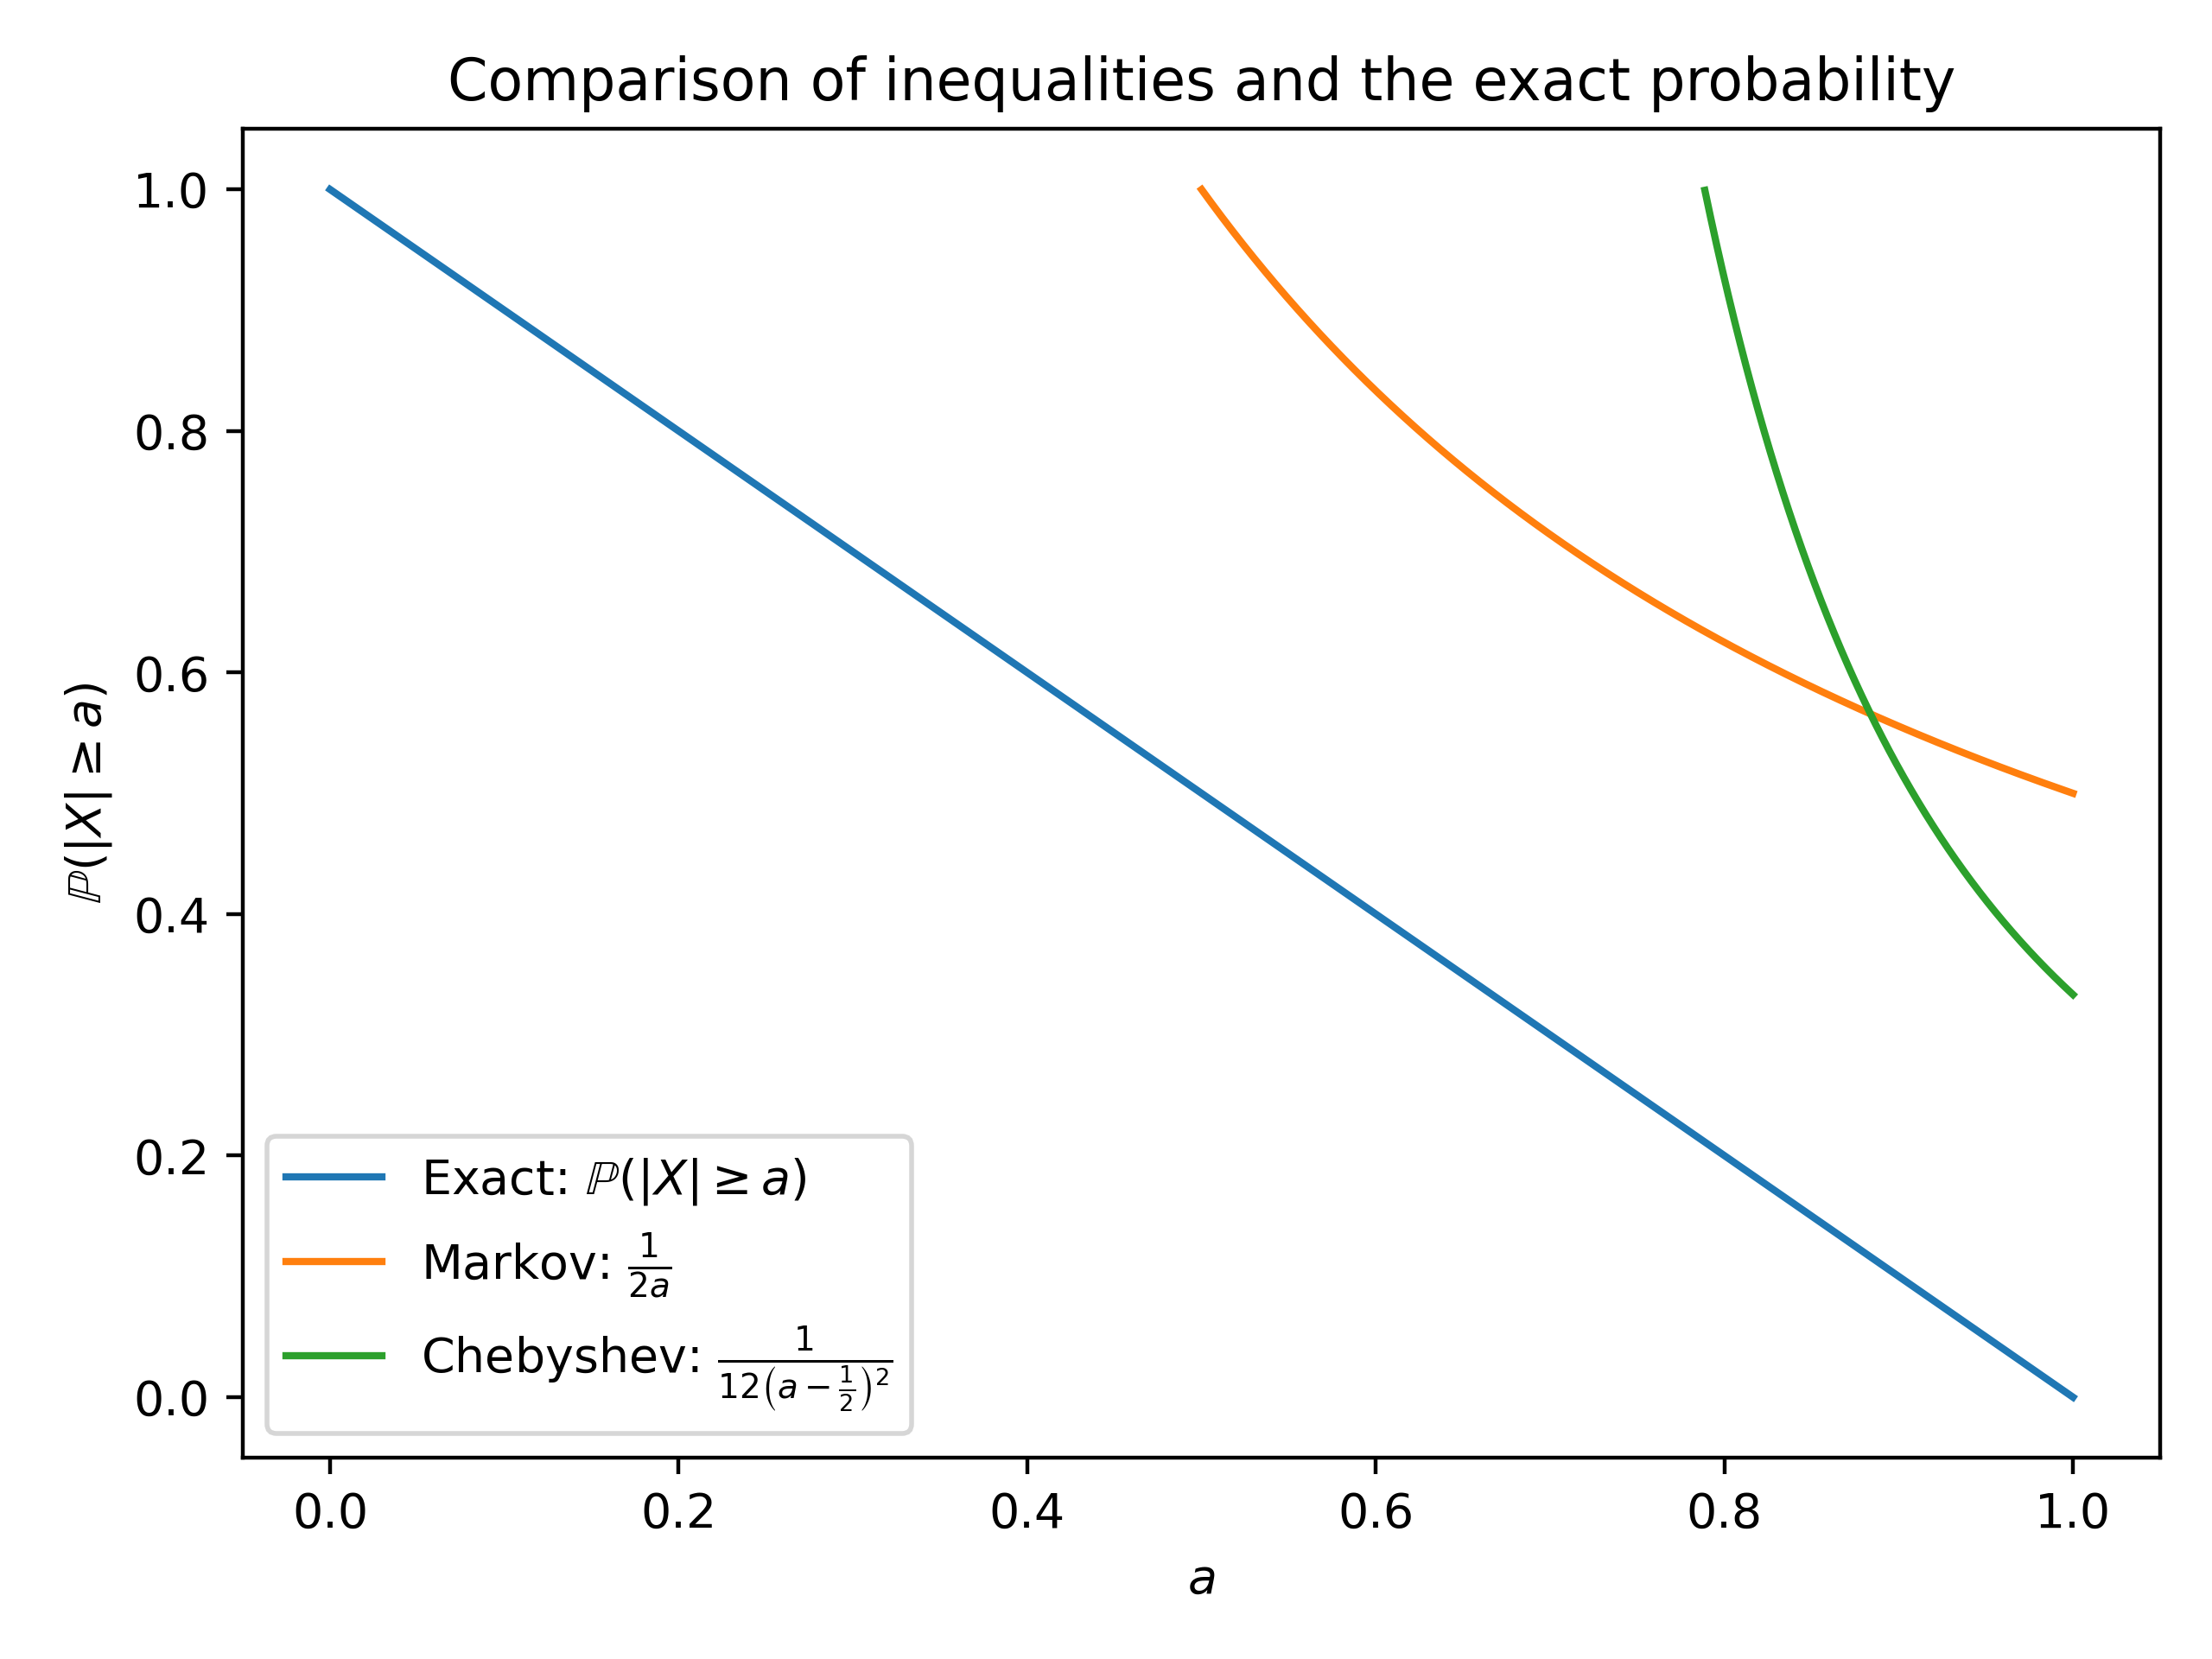
\includegraphics[width=0.6\textwidth]{inequalities}
\end{figure}

\item

Use Chebyshev's inequality to show that the probability that in $n$ throws
of a fair die the number of sixes lies between
\begin{align*}
\frac{1}{6}n - \sqrt{n} & & \text{and} & & \frac{1}{6}n + \sqrt{n}
\end{align*}
is at least $\frac{31}{36}$.

Let $X$ be the number of throws of a fair die that land on six.

Note that $X \sim B\left(n, \frac{1}{6} \right)$. We can therefore use the expression for the variance of a binomial
distribution:

\[
\begin{split}
Var(X) &= np(1 - p) \\
       &= n \times \frac{1}{6} \times \frac{5}{6} \\
       &= \frac{5n}{36} \\
\end{split}
\]

\[
\begin{split}
\mathbb{P}\left(|X - \mathbb{E}(X)| \geq \sqrt{n}\right) &\leq \frac{Var(X)}{n} \\
\mathbb{P}\left(|X - \frac{1}{6}n| \geq \sqrt{n}\right) &\leq \frac{Var(X)}{n} \\
\mathbb{P}\left(X -\frac{1}{6}n \geq \sqrt{n}\right) \vee \mathbb{P}\left(\frac{1}{6}n - X \leq \sqrt{n}\right) &\leq
 \frac{5n}{36n} \\
\mathbb{P}\left(X \geq \frac{1}{6}n + \sqrt{n}\right) \vee \mathbb{P}\left(X \leq \frac{1}{6}n - \sqrt{n}\right) &\leq
 \frac{5}{36} \\
\mathbb{P}\left(X \leq \frac{1}{6}n + \sqrt{n}\right) \vee \mathbb{P}\left(X \geq \frac{1}{6}n - \sqrt{n}\right) &\geq
 \frac{31}{36} \\
\mathbb{P}\left(\frac{1}{6}n - \sqrt{n} \leq X \leq \frac{1}{6}n + \sqrt{n} \right) &\geq \frac{31}{36} \\
\end{split}
\]

\item

The pair of discrete random variables $(X, Y)$ has joint mass function
\[
\mathbb{P}(X = i, Y = j) = \begin{cases}
                           \theta^{i + j + 1} & \text{ if } i, j \in \{0, 1, 2\} \\
                           0 & \text{ otherwise }
                           \end{cases}
\]

for some value of $\theta$.
Show that $\theta$ satisfies the equation:
\[
\theta + 2\theta^2 + 3\theta^3 + 2\theta^4 + \theta^5 = 1
\]

The sum of all probabilities is 1.
So
\[
\begin{split}
1 &= \sum_{i=0}^2\sum_{j=0}^{2} \mathbb{P}(X = i, Y = j) \\
1 &= \sum_{i=0}^{2} \sum_{j=0}^{2} \theta^{i + j + 1} \\
1 &= \theta + 2\theta^2 + 3\theta^3 + 2\theta^4 + \theta^5 \\
\end{split}
\]
As required

Find the marginal mass function of $X$ in terms of $\theta$.
\[
\begin{split}
\mathbb{P}(X = i)
&= \sum_{j=0}^{2} \theta^{i + j + 1} \\
&= \theta^{1 + i}(1 + \theta + \theta^2) \\
\end{split}
\]

Show that
\[
\mathbb{E}(XY) = \theta^3 + 4\theta^4 + 4\theta^5
\]
and
\[
\mathbb{E}(X) = \theta^2 + 3\theta^3 + 3\theta^4 + 2\theta^5
\]

\[
\begin{split}
\mathbb{E}(XY) &= \sum^{2, 2}_{x=0, y=0} xy\mathbb{P}(X = x, Y = y) \\
&= 1\mathbb{P}(X=1,Y=1) + 2(\mathbb{P}(X=1,Y=2) + \mathbb{P}(X=2,Y=1)) + 4(\mathbb{P}(X=2,Y=2)) \\
&= \theta^3 + 4\theta^3 + 4\theta^5 \\
\end{split}
\]

\[
\begin{split}
\mathbb{E}(X) &= \sum^{2}_{x=0} x\mathbb{P}(X=x) \\
&= 1\mathbb{P}(X=1) + 2\mathbb{P}(X=2) \\
&= \theta^2 + \theta^3 + \theta^4 + 2\theta^3 + 2\theta^4 + 2\theta^5 \\
&= \theta^2 + 3\theta^3 + 3\theta^4 + 2\theta^5 \\
\end{split}
\]

\item

Plot the distribution of the sum of 10000 coins that are independent,
with $p(\text{heads}) = 0.7$.
Compute the answer either empirically or in closed form.
Now generate the following: flip the first coin with $p(\text{heads}) = 0.7$.
Then for each of the next 9999 coins, with probability $0.99$, use the previous result as this coin,
and with probability $0.01$ flip a nwe coin with $p(\text{heads}) = 0.7$.
Sum all of them.
Repeat this experiment as many times to estimate the distribution.
Plot.
Comment on the result.

\begin{figure}[H]
\centering
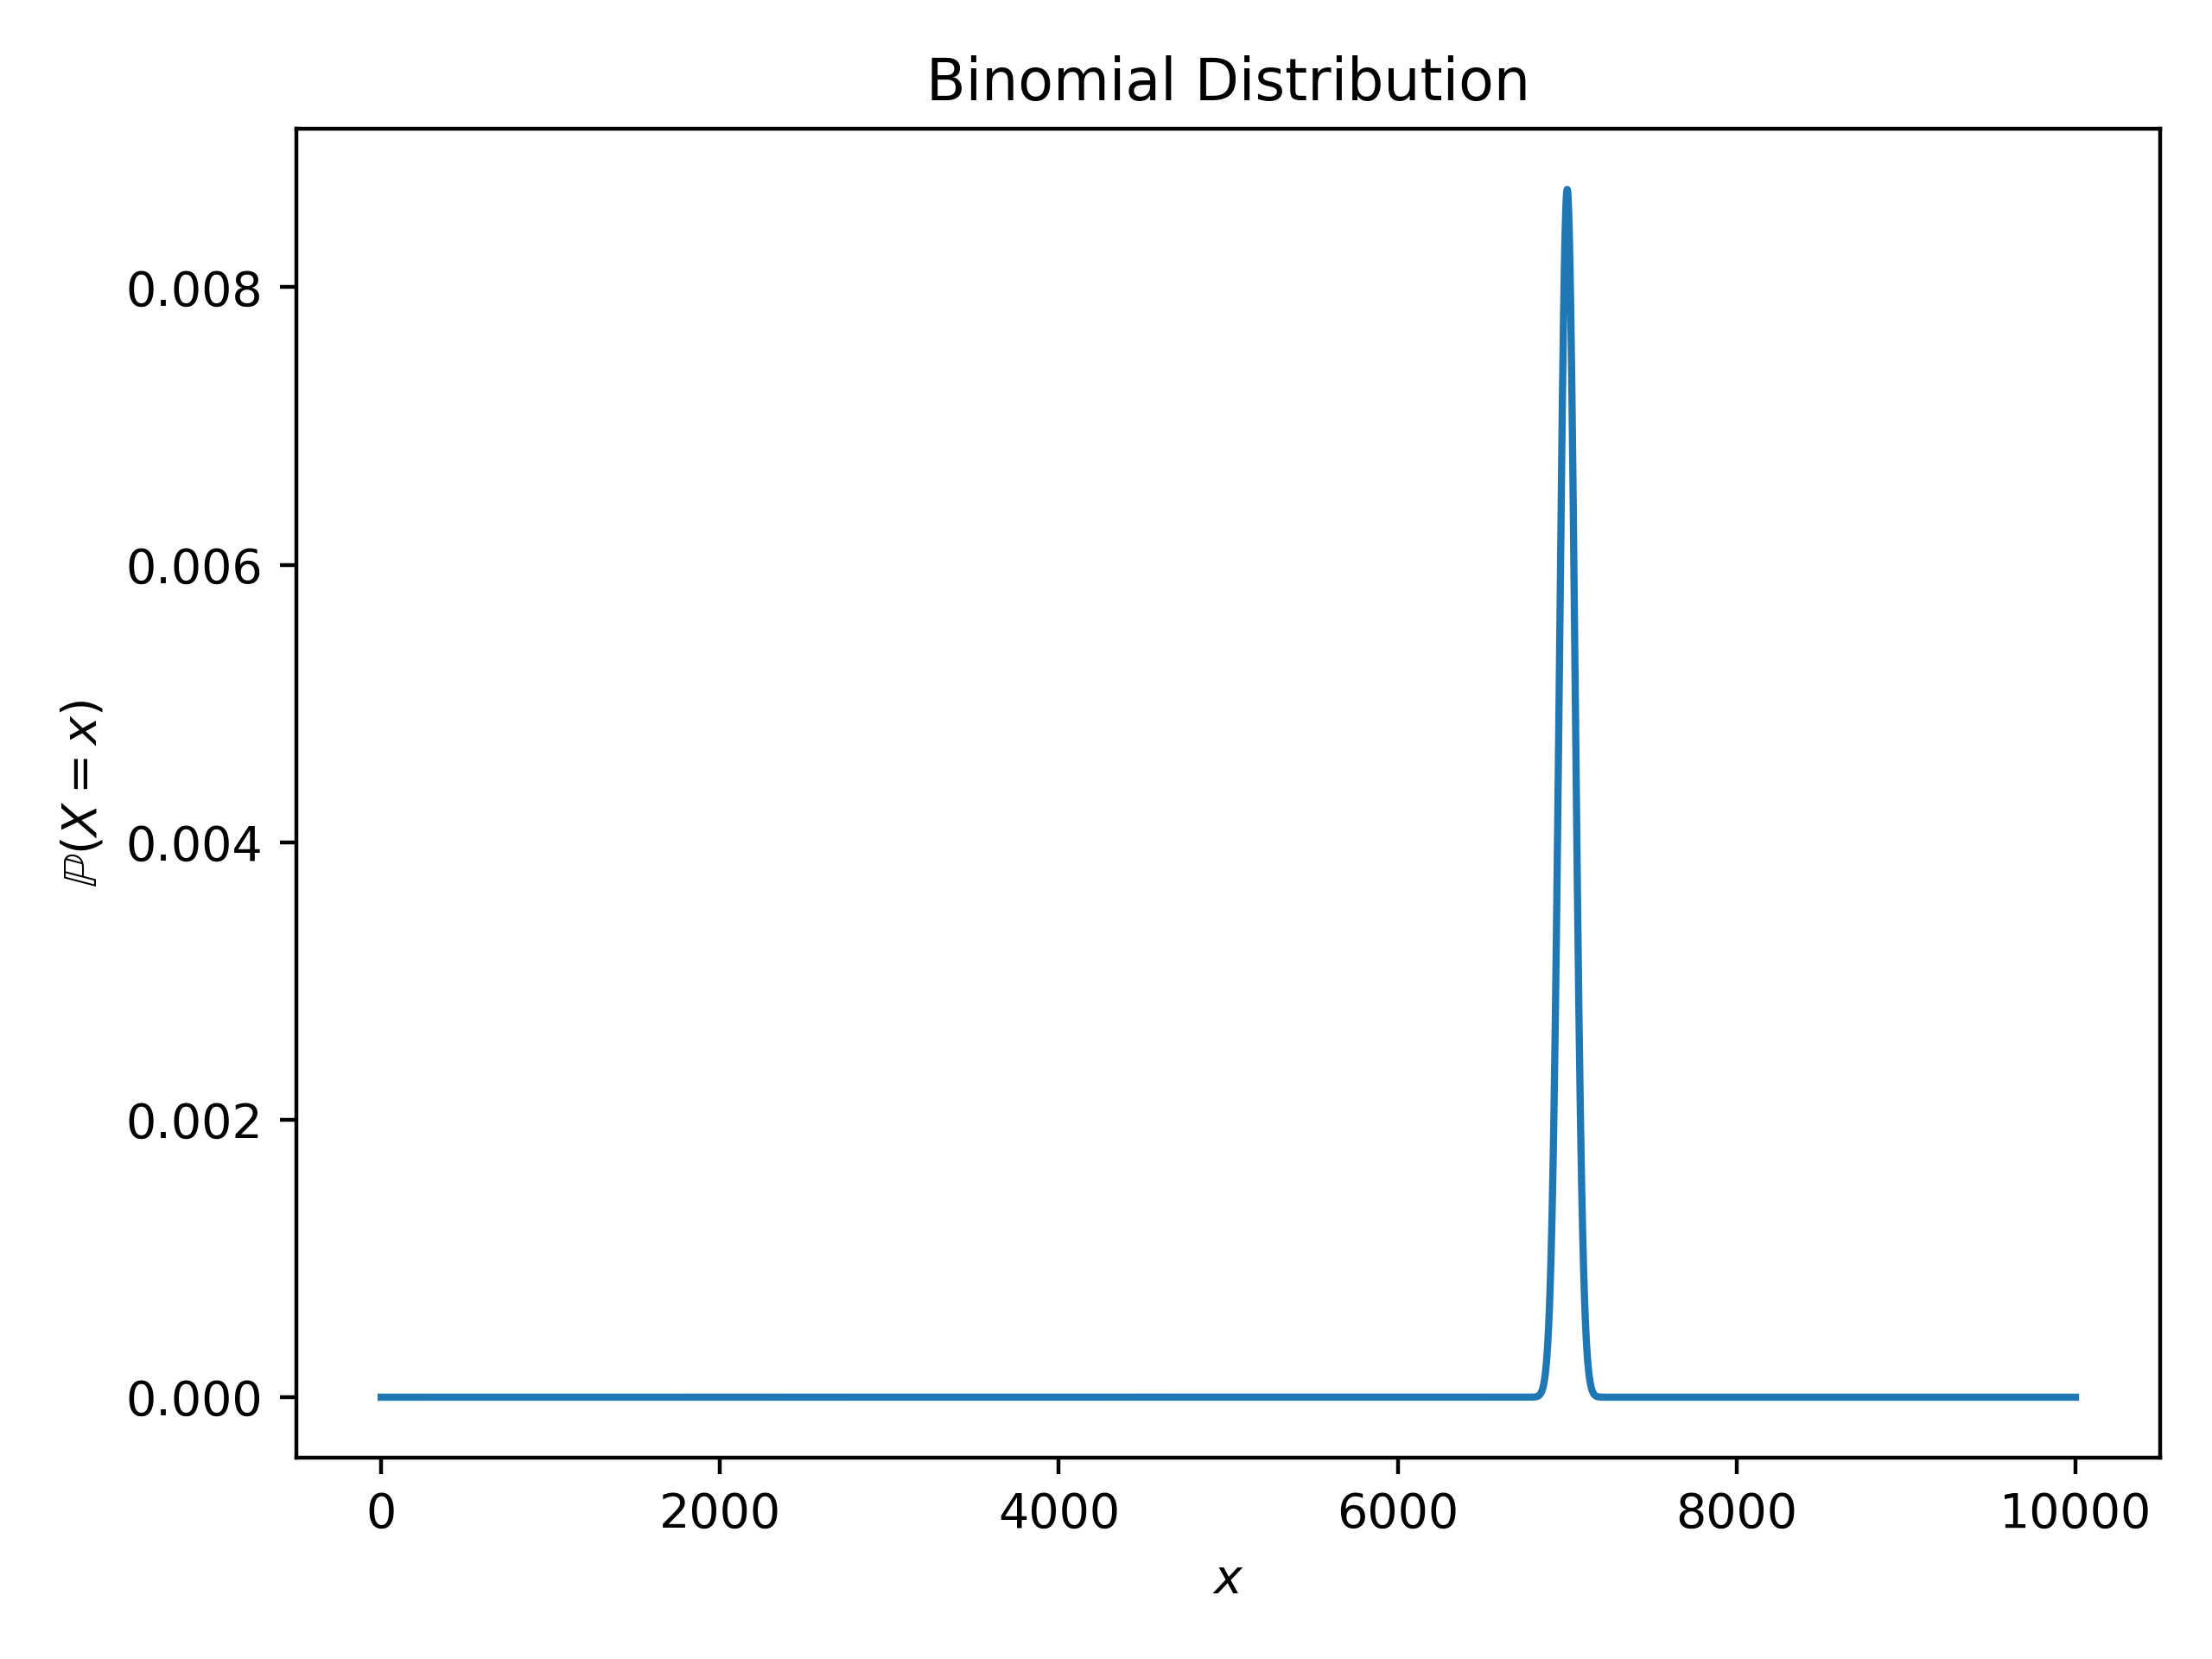
\includegraphics[width=0.6\textwidth]{normabinomial}
\end{figure}

The distribution of the sum of 10000 coin flips that are independent with $p(\text{heads}) = 0.7$ is:
\[
X \sim B(10000, 0.7)
\]

\begin{figure}[H]
\centering
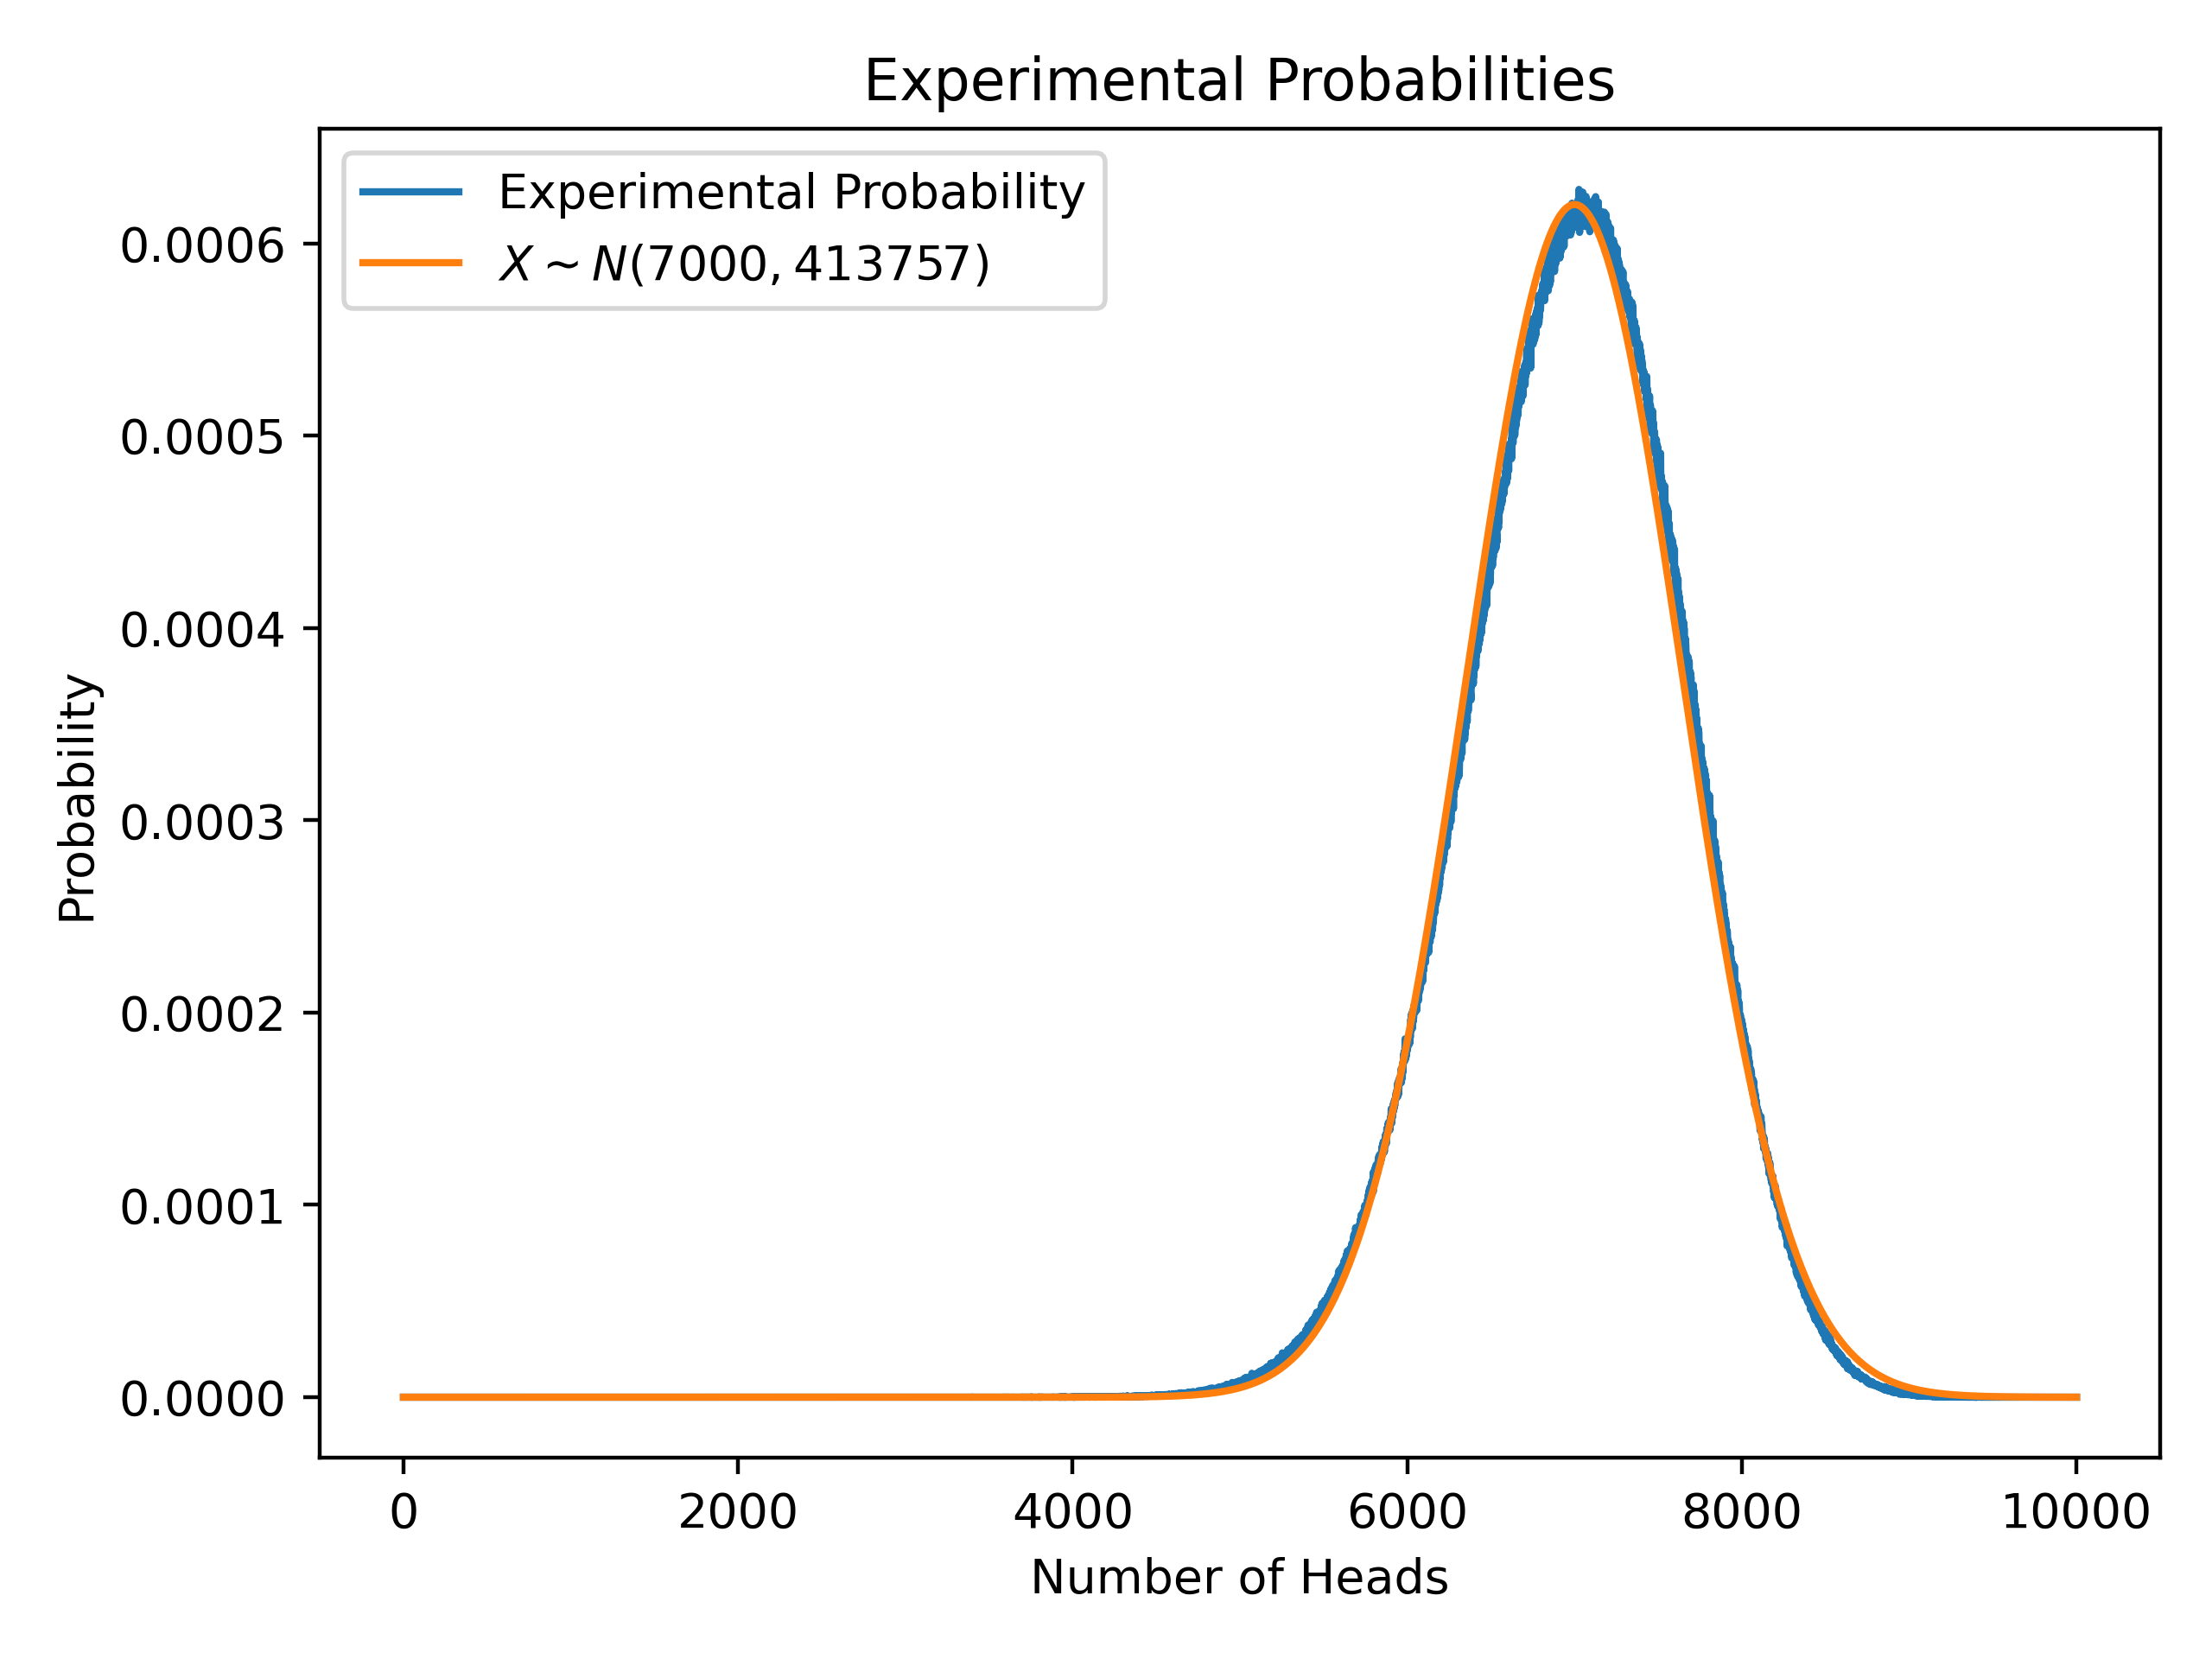
\includegraphics[width=0.6\textwidth]{experimental_prob}
\caption{Graph with 32 million test runs}
\end{figure}

The distribution of the sum of the second situation can be approximated by:
\[
X \sim N(7000, 413757)
\]

This has the same mean as the original binomial distribution, however the variance
is significantly higher.
Normal distributions can model most situations which are not highly skewed.
This is not highly skewed and so can be modelled by a normal distribution.

Here is a proof of the mean of the second situation:

Let $\nu_i$ be the outcome of the $i^{\text{th}}$ coin for $1 \leq i \leq 10000$.

Prove for all $i \in [1, 10000]$, $\mathbb{E}(\nu_i) = 0.7$
\[
\mathbb{E}(\nu_1) = 0.7 \times 1 + 0.3 \times 0 = 0.7
\]

So $\mathbb{E}(\nu_1) = 0.7$

Assume now that the statement also holds true for $\nu_k$:
\[
\begin{split}
\mathbb{E}(\nu_{k + 1})
&= 0.99 \times \mathbb{E}(\nu_k) + 0.01 \times 0.7 \times 1 + 0.01 \times 0.3 \times 0 \\
&= (0.99 + 0.01) \times 0.7 \\
&= 0.7 \\
\end{split}
\]
So if $\mathbb{E}(\nu_k) = 0.7$, then $\mathbb{E}(\nu_{k + 1}) = 0.7$. Since $\mathbb{E}(\nu_1) = 0.7$, for all $n \in
[1, 10000]$, $\mathbb{E}(\nu_n) = 0.7$.

Let $Y$ be the random variable described.
\[
\begin{split}
\mathbb{E}(Y) &= \mathbb{E}\left( i \right) \\
&= \sum^{10000}_{i=1} \mathbb{E}(\nu_i) \text{ by linearity of expectation }\\
&= \sum^{10000}_{i=1} 0.7 \\
&= 7000
\end{split}
\]
So the mean of $Y$ is 7000. As required.

\item

Given a collection of random variables that are pairwise independent (namely,
every pair of random variables are independent), are they jointly independent?
If not, find a counterexample.

No.

Consider the three variables $X, Y, Z$ defined by:
\begin{gather*}
X \sim Bernoulli\left(\frac{1}{2}\right) \\
Y \sim Bernoulli\left( \frac{1}{2} \right) \\
Z = \begin{cases}
    1 & \text{ if } X = Y \\
    0 & \text{ otherwise } \\
    \end{cases}
\end{gather*}

Using these definitions we can see that $X, Y, Z$ are all pairwise independent.\\
However, $\mathbb{P}(Z=1|X=Y=1) = 1 \neq \mathbb{P}(Z=1)$ so they are not jointly independent.

\item

A (potentially) biased coin has probability $p$ of landing heads-up.
A random number $N \sim Po(\lambda)$ of times, you toss the coin.
$N$ is independent of the outcomes of the tosses.
Find the distributions of the numbers $H$ and $T$ denoting the number
of heads and tails obtained respectively.
Also show that $H$ and $T$ are independent.

For some number of total throws $n$; the probability density $f$ of $H$ is given by:
\[
f(i) = \begin{pmatrix} n \\ i \\ \end{pmatrix} p^i(1-p)^{n - i}
\]
Now consider that $n \sim Po(\lambda)$.
So the probability density $f$ of $H$ is now given
by:
\[
\begin{split}
f(i) &= \sum^{\infty}_{n=i} \frac{\lambda^n e^{-\lambda}}{n!} \begin{pmatrix} n \\ i \\ \end{pmatrix} p^i (1 - p)^{n -
i} \\
f(i) &= p^i e^{-\lambda}\sum^{\infty}_{n=i} \frac{\lambda^n}{n!} \frac{n!}{i!(n - i)!} (1 - p)^{n - i} \\
f(i) &= \frac{p^i e^{-\lambda}}{i!} \sum^{\infty}_{n=i} \frac{\lambda^i \lambda^{n - i} (1 - p)^{n - i}}{(n - i)!} \\
f(i) &= \frac{(\lambda p)^i e^{-\lambda}}{i!} \sum^{\infty}_{n=0} \frac{(\lambda (1 - p))^n}{n!} \\
f(i) &= \frac{(\lambda p)^i e^{-\lambda}}{i!} e^{\lambda(1 - p)} \\
f(i) &= \frac{(\lambda p)^i e^{-\lambda p)}}{i!} \\
\end{split}
\]
Note that this is the poisson distribution with parameter $\lambda p$.
So $H \sim Po(\lambda p)$.

An analogous argument for $T$ leads to $T \sim Po(\lambda (1 - p))$

To show that $H$ and $T$ are independent, I will show that $\mathbb{P}(H=i \wedge T=j)$ for arbitrary
$i, j$ is equal to $\mathbb{P}(H=i) \times \mathbb{P}(T=j)$.

\[
\begin{split}
\mathbb{P}(H=i \wedge T=j) &= \mathbb{P}(H=i \wedge n=(i + j)) \\
&= \begin{pmatrix} i + j \\ i \\ \end{pmatrix} p^i (1 - p)^{i + j - i} \times \frac{\lambda^{i + j}e^{-\lambda}}{(i + j)
!} \\
&= p^i (1 - p)^j \frac{(i + j)!}{i!j!} \frac{\lambda^i \lambda^j e^{-\lambda p - \lambda (1 - p)}}{(i + j)!} \\
&= \frac{\lambda^i p^i e^{-\lambda p}}{i!} \frac{\lambda^j (1 - p)^j e^{-\lambda(1 - p)}}{j!} \\
&= \frac{(\lambda p)^i e^{-\lambda p}}{i!} \frac{(\lambda(1 - p))^j e^{-\lambda(1 - p)}}{j!} \\
&= \mathbb{P}(H = i)\mathbb{P}(T = j) \\
\end{split}
\]

Since $i$ and $j$ were arbitrary, this holds for all $i, j \in \mathbb{N}$.
So $H$ and $T$ are independent.

\item

There are $n$ different types of prize, and each prize obtained is equally likely
to be any one of the $n$ types.
Let $Y_i$ be the additional number of prizes collected, after obtaining $i$ distinct
types, before a new type of prize is collected.
Show that $Y_i$ has the geometric distribution (and find the parameter) and deduce
the mean number of prizes you will need to collect before you have a complete set.
Also find the mean number of different types of prizes in the first $m$ prizes
received.

Assume we have collected $i < n$ prizes.
If we collect another prize, the probability we have not seen it is $\frac{n - i}{n}$.
If we find a new prize then we have had a success.
If we do not find a new prize then our state has not changed and so the probability on the
next try is still $\frac{n - i}{n}$.
This forms a geometric distribution with parameter $\frac{n - i}{n}$.
So $Y_i \sim Geo\left( \frac{n - i}{n} \right)$ as required.

The expected number of prizes required to collect every prize is:
\[
\begin{split}
\mathbb{E}(X) &= \mathbb{E}(Geo(1)) + \mathbb{E}\left(Geo \left( \frac{n - 1}{n} \right) \right) + \dots +
\mathbb{E}\left( Geo\left(\frac{1}{n} \right) \right) \\
\mathbb{E}(X) &= \sum^{n - 1}_{i=0} \frac{n}{n - i} \\
\mathbb{E}(X) &= n\sum^{n}_{i=1} \frac{1}{i} \\
\mathbb{E}(X) &= nH_n \\
\mathbb{E}(X) &\approx n\ln n \\
\end{split}
\]

If we collect $m$ prizes then we expect to find $i$ different prizes where $m \approx iH_i$.

\item

This question is related to the example loading a container with packets.
Also here, we assume that the packets have weights drawn independently from
a $Exp(0.5)$ distribution.

How large must the capacity of the container be so that we can store at least 40
packets with 99\% probability.

There are two methods this can be done: exact or approximate.

\begin{itemize}

\item By approximating with the normal distribution (my official answer)

The distribution of the sum of $n$ poisson variables with parameter $\lambda$ where $n$ is large can be approximated
by the normal distribution with normal $\frac{n}{\lambda}$ and variance $\frac{n}{\lambda^2}$. So in this case we can
approximate the distribution with $Y \sim N(80, 160)$.

We wish to find the value which the sum has a probability of 0.99 of being below.

\[
\begin{split}
\phi(2.3263\dots) &= 0.99 \Longrightarrow \\
\mathbb{P}(Y \leq \mu + 2.3263 \sigma) &= 0.99 \Longrightarrow \\
\mathbb{P}(Y \leq 109.43\dots) &= 0.99 \\
\end{split}
\]

So by approximating with the normal distribution, the container must have capacity $\geq 109.43$ to $2 D.P$.

\item By using the true distribution (not an official answer -- this is not manageable in an exam)

The sum of $40$ exponential distributions with parameter $\frac{1}{2}$ is given by
$\Gamma\left( 40, \frac{1}{2} \right)$.

So the distribution of the sum of the parameters is given by:
\[
\Gamma\left( 40, \frac{1}{2} \right) = \frac{\frac{1}{2}^{40} x^{-39} e^{-\frac{1}{2} x}}{\Gamma\left(\frac{1}{2}\right)} \\
\]

If the integral between this and some capacity $a$ is 0.99, then there is a $99\%$ probability
we can store 40 packets in the container:
\[
\begin{split}
\gamma_a\left( 40, \frac{1}{2} \right) &= 0.99 \Longrightarrow \\
a &= \gamma^{-1}\left( 40, \frac{1}{2} \right)(0.99) \\
\end{split}
\]
This can be solved numerically and is $112.33$ to $2 D.P.$.

\end{itemize}

\end{enumerate}

\end{document}